\documentclass[10pt,letterpaper]{article}
\textwidth = 6.5in
\textheight = 9in
\hoffset=-.75in
\voffset=-.8in


\usepackage[pass]{geometry}
%\usepackage[hypertex]{hyperref}
\usepackage{hyperref}
\usepackage{lastpage}
\usepackage{fancyhdr}
\usepackage{sectsty}
\usepackage{amsmath}
\usepackage{scrextend}

\usepackage{listings}
\usepackage{xcolor}
\usepackage{graphicx}
\usepackage{epsfig}

%\graphicspath{ {./images/} }
\usepackage{tikz}
\usepackage{tikz-qtree}
\usepackage{tikz-timing}
	\usetikzlibrary{arrows.meta}
	%\usetikztiminglibrary[simple]{advnodes}
	\usetikztiminglibrary{advnodes}
	\usetikzlibrary{automata, positioning, arrows}
\usepackage{enumitem}
\usepackage{placeins}








\sectionfont{\Large\sf\bfseries}
\subsectionfont{\large\sf\bfseries}

\pagestyle{fancy}
% supress normal headings and footters
\fancyhf{}
% remove the heading rule
\renewcommand{\headrulewidth}{0pt}

\lfoot{{\sf\scriptsize Copyright \copyright\ 2020, 2022 John Winans.  All Rights Reserved}\\
{\scriptsize\FooterText}}
%\lfoot{\scriptsize\FooterText}

\rfoot{Page \thepage\ of \pageref*{LastPage}}

% Sub-footer that shows the VCS Header in the lfoot defined above
\ifdefined\GitFileName
    \newcommand{\FooterText}{\tt \GitFileName\\
\GitDescription}
\else
    \newcommand{\FooterText}{\emph{--UNKNOWN--}}
\fi


\setlength{\parindent}{0pt}
\setlength{\parskip}{.51em}


%%%%%%%%%%%%%%%%%%%%%%%%%%%%%%%%%%%%%%%%%%%%%%%%%%%%%%%%%%%%%%%%%%%%
\definecolor{c_lightblue}{HTML}{B0E0FF}
\definecolor{c_lightred}{HTML}{FFE0E0}
\definecolor{c_lightyellow}{HTML}{FFE060}
\definecolor{c_lightgreen}{HTML}{C0FFC0}
\definecolor{c_lightgray}{HTML}{C0C0C0}
%%%%%%%%%%%%%%%%%%%%%%%%%%%%%%%%%%%%%%%%%%%%%%%%%%%%%%%%%%%%%%%%%%%%

%%%%%%%%%%%%%%%%%%%%%%%%%%%%%%%%%%%%%%%%%%%%%%%%%%%%%%%%%%%%%%%%%%%%
%%%%%%%%%%%%%%%%%%%%%%%%%%%%%%%%%%%%%%%%%%%%%%%%%%%%%%%%%%%%%%%%%%%%
%%%%%%%%%%%%%%%%%%%%%%%%%%%%%%%%%%%%%%%%%%%%%%%%%%%%%%%%%%%%%%%%%%%%
%%%%%%%%%%%%%%%%%%%%%%%%%%%%%%%%%%%%%%%%%%%%%%%%%%%%%%%%%%%%%%%%%%%%
%%%%%%%%%%%%%%%%%%%%%%%%%%%%%%%%%%%%%%%%%%%%%%%%%%%%%%%%%%%%%%%%%%%%

%\title{Finite State Machines}
%\date{September 2021}
%\author{John Winans}

\begin{document}
%\maketitle
\thispagestyle{fancy}

\begin{center}
{\huge Finite State Machines}
\end{center}
\vspace{.5in}

In a manner similar to a synchronous counter, a general FSM 
(Finite State Machine) may be constructed by determining the {\em next state}
from the {\em current state} plus, optionally, any other additional inputs 
that the system may have.

There are two different styles of creating state machines: {\em Moore} and {\em Mealy}.




%%%%%%%%%%%%%%%%%%%%%%%%%%%%%%%%%%%%%%%%%%%%%%%%%%%%%%%%%%%%%%%%%%%%%%%%%%%%%
\section{Moore State Machines}

In a Moore state machine, the state itself is directly mapped to the output signals.

%%%%%%%%%%%%%%%%%%%%%%%%%%%%%%%%%%%%%%%%%%%%%%%%%%%%%%%%%%%%%%%%%%%%%%%%%%%%%
\begin{figure}[ht]
\centering

\scalebox{.75}{\input{moore.pdf_t}}
%\scalebox{.75}{\includegraphics[type=eps,ext=.eps,read=.eps]{{moore.pstex}}

\caption{Moore FSM Block Diagram}
\label{wav:moore.block.diagram}
\end{figure}
%%%%%%%%%%%%%%%%%%%%%%%%%%%%%%%%%%%%%%%%%%%%%%%%%%%%%%%%%%%%%%%%%%%%%%%%%%%%%

\subsection{Synchronous Counter}

Consider a a synchronous counter with an {\em enable} input that when 
high, allows the counter to advance and that when low prevents the counter
from advancing.

State table:

\begin{center}
\begin{tabular}{|cc|c||cc|cc|}
\hline
\multicolumn{2}{|c|}{Current State} &  Input & \multicolumn{2}{|c|}{Next State} & \multicolumn{2}{|c|}{Output} \\
$S_1$ & $S_0$ & $E$ & $N_1$ & $N_0$ & $Q_1$ & $Q_0$ \\
\hline
\hline
0 & 0 & 0 & 0 & 0 &  0 & 0\\
0 & 0 & 1 & 0 & 1 &  0 & 0\\
0 & 1 & 0 & 0 & 1 &  0 & 1\\
0 & 1 & 1 & 1 & 0 &  0 & 1\\
1 & 0 & 0 & 1 & 0 &  1 & 0\\
1 & 0 & 1 & 1 & 1 &  1 & 0\\
1 & 1 & 0 & 1 & 1 &  1 & 1\\
1 & 1 & 1 & 0 & 0 &  1 & 1\\
\hline
\end{tabular}
\end{center}

Boolean functions for the next state in SOP form:

\begin{align}
N_1	& = (\overline{S_1} \land S_0 \land E) \lor
		(S_1 \land \overline{S_0} \land \overline{E}) \lor
		(S_1 \land \overline{S_0} \land E) \lor
		(S_1 \land S_0 \land \overline{E}) \\
N_0	& = (\overline{S_1} \land \overline{S_0} \land E) \lor
		(\overline{S_1} \land S_0 \land \overline{E}) \lor
		(S_1 \land \overline{S_0} \land E) \lor
		(S_1 \land S_0 \land \overline{E})\\
Q_0 & = S_0\\
Q_1 & = S_1
\end{align}

Note that the output of this counter is the value of the {\em state} itself.

%%%%%%%%%%%%%%%%%%%%%%%%%%%%%%%%%%%%%%%%%%%%%%%%%%%%%%%%%%%%%%%%%%%%%%%%%%%%%
%\begin{figure}[ht]
%\centering
%
%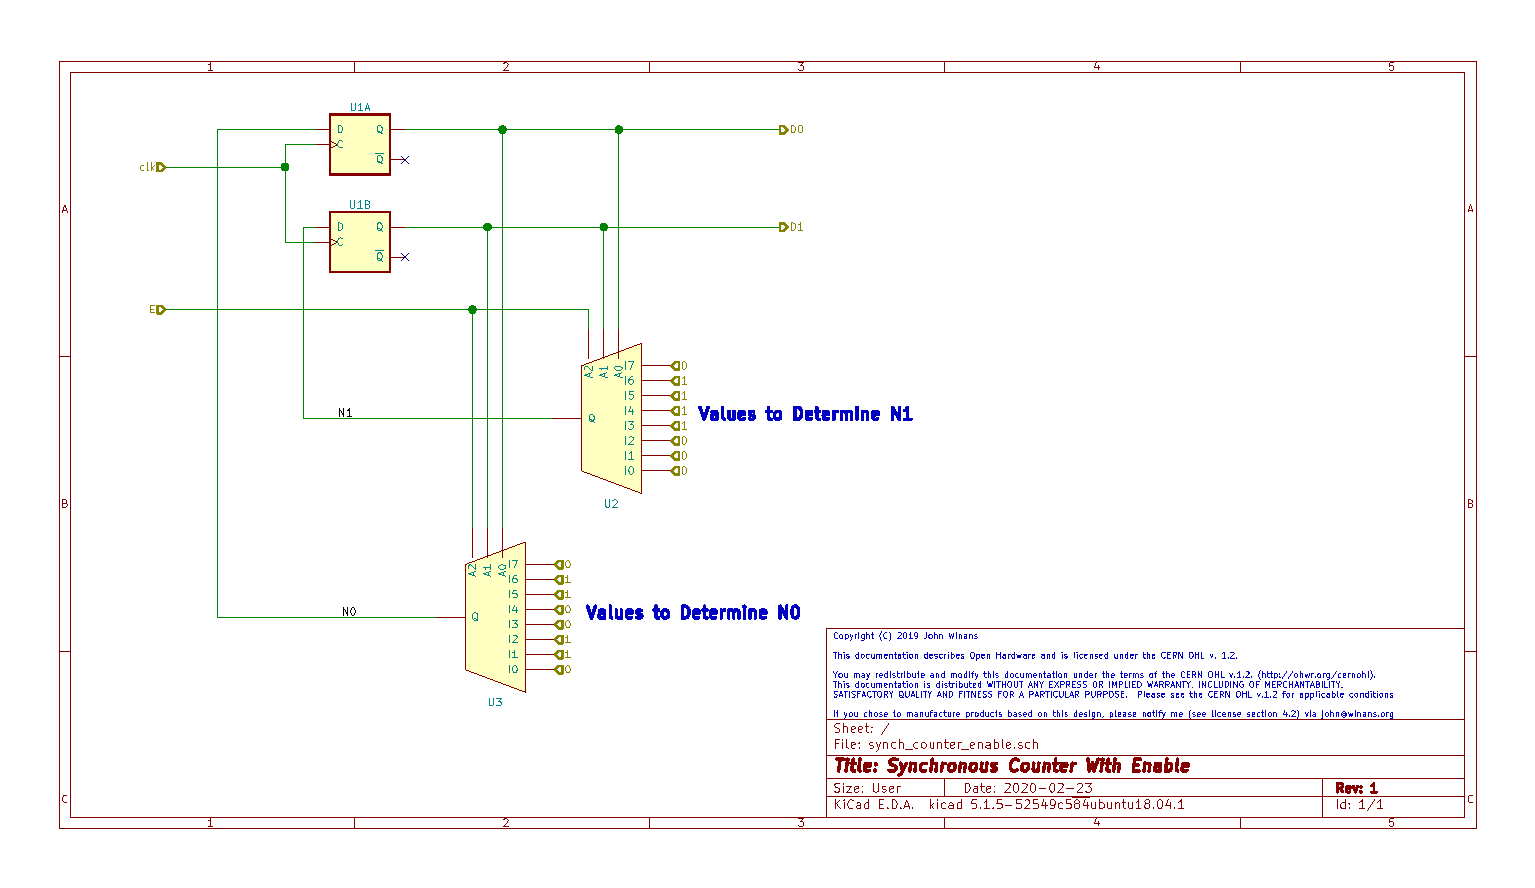
\includegraphics[width=\textwidth]{synch_counter_enable/synch_counter_enable.pdf}
%
%\caption{Synchronous Counter With Enable Schematic}
%\label{sch:synchronous.counter.enable}
%\end{figure}
%%%%%%%%%%%%%%%%%%%%%%%%%%%%%%%%%%%%%%%%%%%%%%%%%%%%%%%%%%%%%%%%%%%%%%%%%%%%%


%%%%%%%%%%%%%%%%%%%%%%%%%%%%%%%%%%%%%%%%%%%%%%%%%%%%%%%%%%%%%%%%%%%%%%%%%%%%%
\begin{figure}[ht] 
\centering 
\begin{tikzpicture} [
	->,  % makes the edges directed
	>=stealth, % makes the arrow heads bold
	node distance=2cm, % specifies the minimum distance between two nodes. Change if necessary.
	every state/.style={thick, fill=gray!10}, % sets the properties for each 'state' node
	initial text=$ $, % sets the text that appears on the start arrow
	]
	\node[state, initial] (s0) {00/00};
	\node[state, right of=s0] (s1) {01/01};
	\node[state, below of=s1] (s2) {10/10};
	\node[state, left of=s2] (s3) {11/11};
	\draw
		(s0) edge[loop above] node{0} (s0)
		(s0) edge[bend left, above] node{1} (s1)

		(s1) edge[loop above] node{0} (s1)
		(s1) edge[bend left, right] node{1} (s2)

		(s2) edge[loop below] node{0} (s2)
		(s2) edge[bend left, below] node{1} (s3)

		(s3) edge[loop below] node{0} (s3)
		(s3) edge[bend left, left] node{1} (s0)
	;
\end{tikzpicture}
\caption{Synchronous Counter With Enable State Diagram}
\label{fsm:synchronous.counter.enable}
\end{figure}
%%%%%%%%%%%%%%%%%%%%%%%%%%%%%%%%%%%%%%%%%%%%%%%%%%%%%%%%%%%%%%%%%%%%%%%%%%%%%

When we draw a Moore style state diagram, the nodes are labeled with the
output values from the circuit and the edges include a value representing
any inputs.

In Fig~\ref{fsm:synchronous.counter.enable} the state in the lower-left part of 
the diagram represents state $11$ and shows every possible value of the circuit's
inputs (in this case, only $E$) along the edges that exit from that state.
The edge that loops from state $11$ back to itself, for example, represents 
how the circuit will react to the clock signal when $E$ is low.  The edge
that exits from state $11$ to state $00$ represents how the circuit will react 
to the clock signal when $E$ is high.









%%%%%%%%%%%%%%%%%%%%%%%%%%%%%%%%%%%%%%%%%%%%%%%%%%%%%%%%%%%%%%%%%%%%%%%%%%%%%
\subsection{Message Recognizer}

Rather than counting {\em in order} and providing a mechanism for starting and
stopping the counting, a circuit may be created that uses external inputs
to change the order in which the counting is done.  Additionally, the
count value can be used for more than determining the next state.

Consider a circuit designed to recognize a message (011) that arrives over 
time on signal $D$ as a series of samples taken on the falling edges of a 
clock signal and generates a high level on signal $Q$ when so recognized.

State table:

\begin{center}
\begin{tabular}{|cc|c||cc|c|}
\hline
\multicolumn{2}{|c|}{Current State} & Input & \multicolumn{2}{|c|}{Next State} & Output \\
$S_1$ & $S_0$ & $D$ & $N_1$ & $N_0$ & $Q$ \\
\hline
\hline
0 & 0 &  0  & 0 & 1 &  0\\
0 & 0 &  1  & 0 & 0 &  0\\
0 & 1 &  0  & 0 & 1 &  0\\
0 & 1 &  1  & 1 & 0 &  0\\
1 & 0 &  0  & 0 & 1 &  0\\
1 & 0 &  1  & 1 & 1 &  0\\
1 & 1 &  0  & 0 & 1 &  1\\
1 & 1 &  1  & 0 & 0 &  1\\
\hline
\end{tabular}
\end{center}

Boolean functions for the next state in SOP form:

\begin{align}
N_1	& = (\overline{S_1} \land S_0 \land D) \lor
%		(S_1 \land \overline{S_0} \land \overline{D}) \lor
		(S_1 \land \overline{S_0} \land D) \\
N_0	& = (\overline{S_1} \land \overline{S_0} \land \overline{D}) \lor
		(\overline{S_1} \land S_0 \land \overline{D}) \lor
		(S_1 \land \overline{S_0} \land \overline{D}) \lor
		(S_1 \land \overline{S_0} \land D) \lor
		(S_1 \land S_0 \land \overline{D})\\
Q &= S_1 \land S_0
\end{align}

%%%%%%%%%%%%%%%%%%%%%%%%%%%%%%%%%%%%%%%%%%%%%%%%%%%%%%%%%%%%%%%%%%%%%%%%%%%%%
\begin{figure}[ht]
\centering
\begin{tikztimingtable} [yscale=1.5,xscale=3,timing/slope=0.05,timing/coldist=1pt]
 state	& { DD{}6{DD{}}DD } \\ %SSSSSSSSSSSSSSS }\\
 $clk$	& { LHLHLHLHLHLHLHLH }\\
 $D$	& { LLLLLHHHHLLLLLLL }\\
 $Q$	& { LLLLLLLLHHLLLLLL }\\
\extracode
 \makeatletter
 \begin{pgfonlayer}{background}
  \begin{scope}[gray,semitransparent,semithick]
        \vertlines{0,2,...,\twidth}
  \end{scope}
        \foreach \n [count=\i from 0] in {0,1,...,\twidth}
            \draw (\n,-\nrows*2+1.5) -- +(0,-.2)
                node [below,inner sep=2pt] {\scalebox{.75}{\tiny\i}};
%    \draw [fill=c_lightgray,c_lightgray] (0,-4) rectangle (2,-3);
 \end{pgfonlayer}
	\draw[blue] (1,.5) node{00};
	\draw[blue] (3,.5) node{01};
	\draw[blue] (5,.5) node{01};
	\draw[blue] (7,.5) node{10};
	\draw[blue] (9,.5) node{11};
	\draw[blue] (11,.5) node{01};
	\draw[blue] (13,.5) node{01};
	\draw[blue] (15,.5) node{01};
\end{tikztimingtable}

\caption{Message 0 1 1 Recognizer Moore FSM Waveform}
\label{wav:moore.message.011}
\end{figure}
%%%%%%%%%%%%%%%%%%%%%%%%%%%%%%%%%%%%%%%%%%%%%%%%%%%%%%%%%%%%%%%%%%%%%%%%%%%%%



%%%%%%%%%%%%%%%%%%%%%%%%%%%%%%%%%%%%%%%%%%%%%%%%%%%%%%%%%%%%%%%%%%%%%%%%%%%%%
\begin{figure}[ht] 
\centering 
\begin{tikzpicture} [
	->,  % makes the edges directed
	>=stealth, % makes the arrow heads bold
	node distance=3cm, % specifies the minimum distance between two nodes. Change if necessary.
	every state/.style={thick, fill=gray!10}, % sets the properties for each 'state' node
	initial text=$ $, % sets the text that appears on the start arrow
	]
	\node[state, initial] (s0) {00/0};
	\node[state, right of=s0] (s1) {01/0};
	\node[state, right of=s1] (s2) {10/0};
	\node[state, right of=s2] (s3) {11/1};
	\draw
		(s0) edge[loop above] node{1} (s0)
		(s0) edge[bend left, above] node{0} (s1)

		(s1) edge[loop above] node{0} (s1)
		(s1) edge[bend left, above] node{1} (s2)

		(s2) edge[bend left, above] node{0} (s1)
		(s2) edge[bend left, above] node{1} (s3)

		(s3) edge[bend left, above] node{0} (s1)
		(s3) edge[bend left, below] node{1} (s0)
	;
\end{tikzpicture}
\caption{Message 0 1 1 Recognizer Moore FSM State Diagram}
\label{fsm:moore.message.011}
\end{figure}
%%%%%%%%%%%%%%%%%%%%%%%%%%%%%%%%%%%%%%%%%%%%%%%%%%%%%%%%%%%%%%%%%%%%%%%%%%%%%

%%%%%%%%%%%%%%%%%%%%%%%%%%%%%%%%%%%%%%%%%%%%%%%%%%%%%%%%%%%%%%%%%%%%%%%%%%%%%
\begin{figure}[ht]
\centering
\begin{tikztimingtable} [yscale=1.5,xscale=2,timing/slope=0.05,timing/coldist=1pt]
 state	& { DD{}13{DD{}}DD } \\%15{SS} }\\
 $clk$	& { 15{LH} }\\
 $D$	& { LLLHHLLLLHHLLHHHHLLHHHHHHHHLLL }\\
 $Q$	& { LLLLLLLLLLLLLLLLHHLLLLHHLLLLLL }\\
\extracode
 \makeatletter
 \begin{pgfonlayer}{background}
  \begin{scope}[gray,semitransparent,semithick]
        \vertlines{0,2,...,\twidth}
  \end{scope}
        \foreach \n [count=\i from 0] in {0,1,...,\twidth}
            \draw (\n,-\nrows*2+1.5) -- +(0,-.2)
                node [below,inner sep=2pt] {\scalebox{.75}{\tiny\i}};
%    \draw [fill=c_lightgray,c_lightgray] (0,-4) rectangle (2,-3);
 \end{pgfonlayer}
	\draw[blue] (1,.5) node{00};
	\draw[blue] (3,.5) node{01};
	\draw[blue] (5,.5) node{10};
	\draw[blue] (7,.5) node{01};
	\draw[blue] (9,.5) node{01};
	\draw[blue] (11,.5) node{10};
	\draw[blue] (13,.5) node{01};
	\draw[blue] (15,.5) node{10};
	\draw[blue] (17,.5) node{11};
	\draw[blue] (19,.5) node{01};
	\draw[blue] (21,.5) node{10};
	\draw[blue] (23,.5) node{11};
	\draw[blue] (25,.5) node{00};
	\draw[blue] (27,.5) node{00};
	\draw[blue] (29,.5) node{01};
\end{tikztimingtable}

\caption{Message 0 1 1 Recognizer Moore FSM All Possible Transitions}
\label{wav:moore.message.011.all}
\end{figure}
%%%%%%%%%%%%%%%%%%%%%%%%%%%%%%%%%%%%%%%%%%%%%%%%%%%%%%%%%%%%%%%%%%%%%%%%%%%%%

%%%%%%%%%%%%%%%%%%%%%%%%%%%%%%%%%%%%%%%%%%%%%%%%%%%%%%%%%%%%%%%%%%%%%%%%%%%%%
\begin{figure}[ht]
\centering
\begin{tikztimingtable} [yscale=1.5,xscale=2,timing/slope=0.05,timing/coldist=1pt]
 state	& { DD{}13{DD{}}DD } \\%15{SS} }\\
 $clk$	& { 15{LH} }\\
 $D$	& { LLLHHL.25L.25H.25L.25HLLHHLLH.25H.25L.25H.25LHHLLHHHHHHHHLLL }\\
 $Q$	& { LLLLLLLLLLLLLLLLHHLLLLHHLLLLLL }\\
\extracode
 \makeatletter
 \begin{pgfonlayer}{background}
  \begin{scope}[gray,semitransparent,semithick]
        \vertlines{0,2,...,\twidth}
  \end{scope}
        \foreach \n [count=\i from 0] in {0,1,...,\twidth}
            \draw (\n,-\nrows*2+1.5) -- +(0,-.2)
                node [below,inner sep=2pt] {\scalebox{.75}{\tiny\i}};
%    \draw [fill=c_lightgray,c_lightgray] (0,-4) rectangle (2,-3);
 \end{pgfonlayer}
	\draw[blue] (1,.5) node{00};
	\draw[blue] (3,.5) node{01};
	\draw[blue] (5,.5) node{10};
	\draw[blue] (7,.5) node{01};
	\draw[blue] (9,.5) node{01};
	\draw[blue] (11,.5) node{10};
	\draw[blue] (13,.5) node{01};
	\draw[blue] (15,.5) node{10};
	\draw[blue] (17,.5) node{11};
	\draw[blue] (19,.5) node{01};
	\draw[blue] (21,.5) node{10};
	\draw[blue] (23,.5) node{11};
	\draw[blue] (25,.5) node{00};
	\draw[blue] (27,.5) node{00};
	\draw[blue] (29,.5) node{01};
\end{tikztimingtable}

\caption{Message 0 1 1 Recognizer Moore FSM With Glitches}
\label{wav:moore.message.011.glitch}
\end{figure}

%%%%%%%%%%%%%%%%%%%%%%%%%%%%%%%%%%%%%%%%%%%%%%%%%%%%%%%%%%%%%%%%%%%%%%%%%%%%%

\begin{figure}[ht]
\centering
\scalebox{.75}{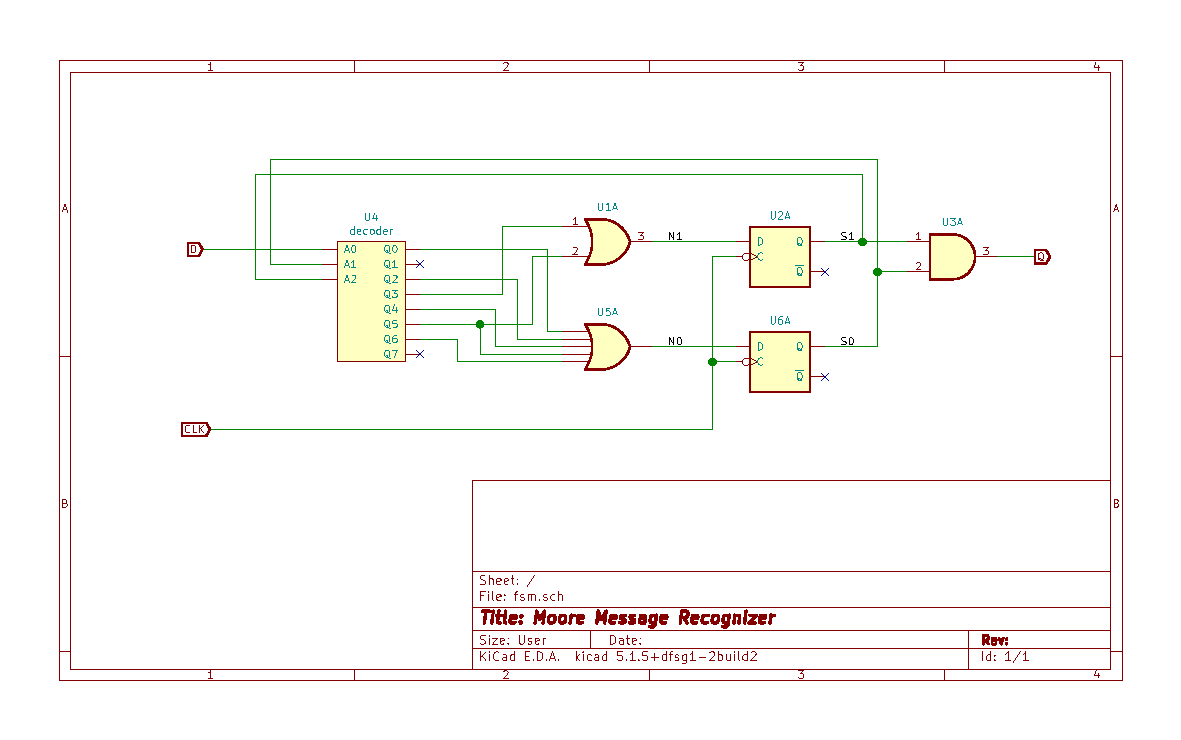
\includegraphics[]{moore/fsm.pdf}}
\caption{Message 0 1 1 Recognizer Moore FSM Schematic}
\label{schematic:moore.message.011}
\end{figure}


\FloatBarrier
\newpage

%%%%%%%%%%%%%%%%%%%%%%%%%%%%%%%%%%%%%%%%%%%%%%%%%%%%%%%%%%%%%%%%%%%%%%%%%%%%%
\section{Mealy State Machines}

In contrast to a Moore state machine, a Mealy state machine is allowed to 
generate output signals from the current state as well as the input signals.

The result is that the outputs from a Mealy state machine can change
asynchronously (if/when the inputs change.)
Like the ripple counter, this can simplify a circuit as long as the 
relationship of the inputs and outputs of the circuit is acceptable 
in the application within which it is used.

One benefit of the Mealy state machine is that it can sometimes require
fewer states.

%%%%%%%%%%%%%%%%%%%%%%%%%%%%%%%%%%%%%%%%%%%%%%%%%%%%%%%%%%%%%%%%%%%%%%%%%%%%%
\begin{figure}[ht]
\centering

\scalebox{.75}{\input{mealy.pdf_t}}

\caption{Mealy FSM Block Diagram}
\label{wav:mealy.block.diagram}
\end{figure}
%%%%%%%%%%%%%%%%%%%%%%%%%%%%%%%%%%%%%%%%%%%%%%%%%%%%%%%%%%%%%%%%%%%%%%%%%%%%%

\subsection{Mealy Message Recognizer}

Note that the output $Q$ in Fig~\ref{wav:moore.message.011} is high when the state is 11. 
In Fig~\ref{wav:mealy.message.011}, $Q$ is high when the state 10 and the input $D$ is high.

State table:

\begin{center}
\begin{tabular}{|cc|c||cc|c|}
\hline
\multicolumn{2}{|c|}{Current State} & Input & \multicolumn{2}{|c|}{Next State} & Output \\
$S_1$ & $S_0$ & $D$ & $N_1$ & $N_0$ & $Q$ \\
\hline
\hline
0 & 0 &  0  & 0 & 1 &  0\\
0 & 0 &  1  & 0 & 0 &  0\\
0 & 1 &  0  & 0 & 1 &  0\\
0 & 1 &  1  & 1 & 0 &  0\\
1 & 0 &  0  & 0 & 1 &  0\\
1 & 0 &  1  & 0 & 0 &  1\\
\hline
\end{tabular}
\end{center}

Note that the state table does not include a state number 3.  
Because this message recognizer only requires states 0, 1 and 2.

Boolean functions for the next state in SOP form:

\begin{align}
N_1	& = (\overline{S_1} \land S_0 \land D)\\
N_0	& = (\overline{S_1} \land \overline{S_0} \land \overline{D}) \lor
		(\overline{S_1} \land S_0 \land \overline{D}) \lor
		(S_1 \land \overline{S_0} \land \overline{D})\\
Q &= S_1 \land \overline{S_0} \land D
\end{align}


%%%%%%%%%%%%%%%%%%%%%%%%%%%%%%%%%%%%%%%%%%%%%%%%%%%%%%%%%%%%%%%%%%%%%%%%%%%%%
\begin{figure}[ht] 
\centering 
\begin{tikzpicture} [
	->,  % makes the edges directed
	>=stealth, % makes the arrow heads bold
	node distance=3cm, % specifies the minimum distance between two nodes. Change if necessary.
	every state/.style={thick, fill=gray!10}, % sets the properties for each 'state' node
	initial text=$ $, % sets the text that appears on the start arrow
	]
	\node[state, initial] (s0) {$00$};
	\node[state, right of=s0] (s1) {$01$};
	\node[state, right of=s1] (s2) {$10$};
	\draw
		(s0) edge[loop above] node{1/0} (s0)
		(s0) edge[bend left, above] node{0/0} (s1)

		(s1) edge[loop above] node{0/0} (s1)
		(s1) edge[bend left, above] node{1/0} (s2)

		(s2) edge[bend left, above] node{0/0} (s1)
		(s2) edge[bend left, below] node{1/1} (s0)
	;
\end{tikzpicture}
\caption{Message 0 1 1 Recognizer Mealy FSM State Diagram}
\label{fsm:mealy.message.011}
\end{figure}
%%%%%%%%%%%%%%%%%%%%%%%%%%%%%%%%%%%%%%%%%%%%%%%%%%%%%%%%%%%%%%%%%%%%%%%%%%%%%

%%%%%%%%%%%%%%%%%%%%%%%%%%%%%%%%%%%%%%%%%%%%%%%%%%%%%%%%%%%%%%%%%%%%%%%%%%%%%
\begin{figure}[ht]
\centering
\begin{tikztimingtable} [yscale=1.5,xscale=2,timing/slope=0.05,timing/coldist=1pt]
 state	& { DD{}13{DD{}}DD } \\ %15{SS} }\\
 $clk$	& { 15{LH} }\\
 $D$	& { LLLHHLLLLHHLLHHHHLLHHHHHHHHLLL }\\
 $Q$	& { LLLLHLLLLLHLLLHHLLLLHHLLLLLLLL }\\
\extracode
 \makeatletter
 \begin{pgfonlayer}{background}
  \begin{scope}[gray,semitransparent,semithick]
        \vertlines{0,2,...,\twidth}
  \end{scope}
        \foreach \n [count=\i from 0] in {0,1,...,\twidth}
            \draw (\n,-\nrows*2+1.5) -- +(0,-.2)
                node [below,inner sep=2pt] {\scalebox{.75}{\tiny\i}};
%    \draw [fill=c_lightgray,c_lightgray] (0,-4) rectangle (2,-3);
 \end{pgfonlayer}
	\draw[blue] (1,.5) node{00};
	\draw[blue] (3,.5) node{01};
	\draw[blue] (5,.5) node{10};
	\draw[blue] (7,.5) node{01};
	\draw[blue] (9,.5) node{01};
	\draw[blue] (11,.5) node{10};
	\draw[blue] (13,.5) node{01};
	\draw[blue] (15,.5) node{10};
	\draw[blue] (17,.5) node{00};
	\draw[blue] (19,.5) node{01};
	\draw[blue] (21,.5) node{10};
	\draw[blue] (23,.5) node{00};
	\draw[blue] (25,.5) node{00};
	\draw[blue] (27,.5) node{00};
	\draw[blue] (29,.5) node{01};
\end{tikztimingtable}

\caption{Message 0 1 1 Recognizer Mealy FSM All Possible Transitions}
\label{wav:mealy.message.011}
\end{figure}
%%%%%%%%%%%%%%%%%%%%%%%%%%%%%%%%%%%%%%%%%%%%%%%%%%%%%%%%%%%%%%%%%%%%%%%%%%%%%

The output of a Mealy state machine can deliver its output sooner than the 
Moore state machine.  
However, the Mealy state machine can also glitch as shown in 
Fig~\ref{wav:mealy.message.011.glitch} in ways that the Moore machine will not.

%%%%%%%%%%%%%%%%%%%%%%%%%%%%%%%%%%%%%%%%%%%%%%%%%%%%%%%%%%%%%%%%%%%%%%%%%%%%%
\begin{figure}[ht]
\centering
\begin{tikztimingtable} [yscale=1.5,xscale=2,timing/slope=0.05,timing/coldist=1pt]
 state	& { DD{}13{DD{}}DD } \\
 $clk$	& { 15{LH} }\\
 $D$	& { LLLHHL.25L.25H.25L.25HLLHHLLH.25H.25L.25H.25LHHLLHHHHHHHHLLL }\\
 $Q$	& { LLLLHLLLLLHLLL.25H.25L.25H.25LHLLLLHHLLLLLLLL }\\
\extracode
 \makeatletter
 \begin{pgfonlayer}{background}
  \begin{scope}[gray,semitransparent,semithick]
        \vertlines{0,2,...,\twidth}
  \end{scope}
        \foreach \n [count=\i from 0] in {0,1,...,\twidth}
            \draw (\n,-\nrows*2+1.5) -- +(0,-.2)
                node [below,inner sep=2pt] {\scalebox{.75}{\tiny\i}};
%    \draw [fill=c_lightgray,c_lightgray] (0,-4) rectangle (2,-3);
 \end{pgfonlayer}
	\draw[blue] (1,.5) node{00};
	\draw[blue] (3,.5) node{01};
	\draw[blue] (5,.5) node{10};
	\draw[blue] (7,.5) node{01};
	\draw[blue] (9,.5) node{01};
	\draw[blue] (11,.5) node{10};
	\draw[blue] (13,.5) node{01};
	\draw[blue] (15,.5) node{10};
	\draw[blue] (17,.5) node{00};
	\draw[blue] (19,.5) node{01};
	\draw[blue] (21,.5) node{10};
	\draw[blue] (23,.5) node{00};
	\draw[blue] (25,.5) node{00};
	\draw[blue] (27,.5) node{00};
	\draw[blue] (29,.5) node{01};
\end{tikztimingtable}

\caption{Message 0 1 1 Recognizer Mealy FSM With Glitches}
\label{wav:mealy.message.011.glitch}
\end{figure}
%%%%%%%%%%%%%%%%%%%%%%%%%%%%%%%%%%%%%%%%%%%%%%%%%%%%%%%%%%%%%%%%%%%%%%%%%%%%%

\begin{figure}[ht]
\centering
\scalebox{.75}{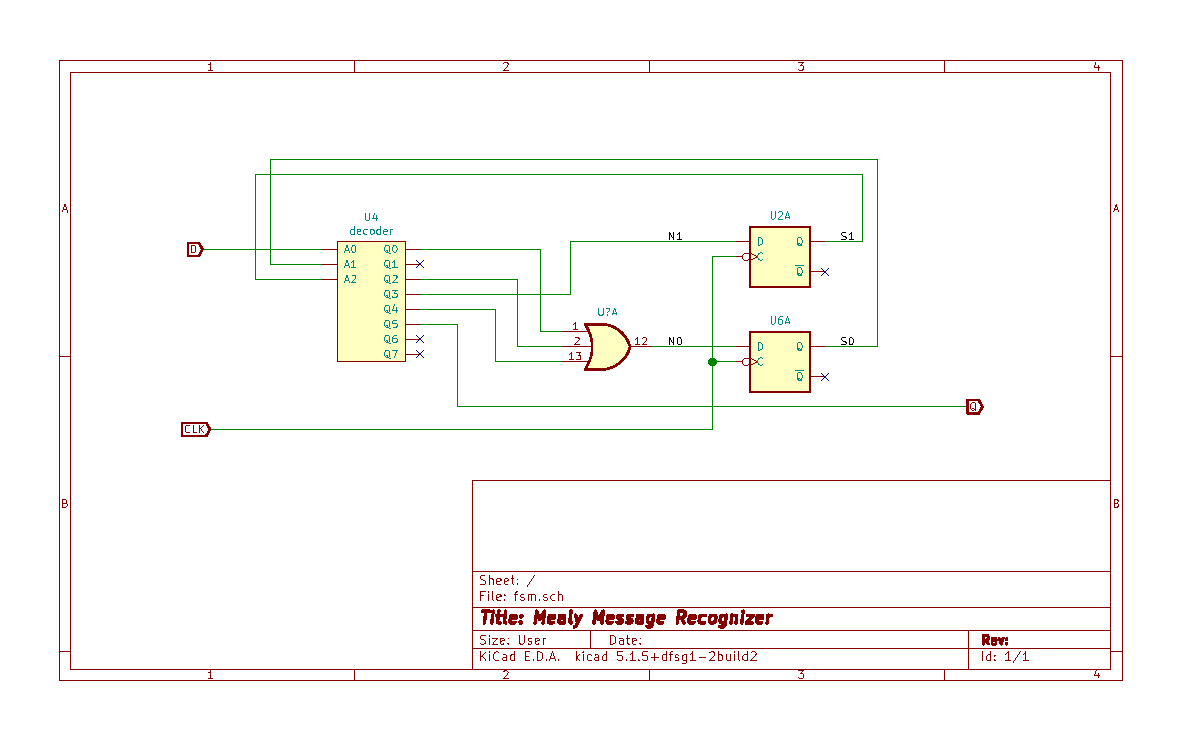
\includegraphics[]{mealy/fsm.pdf}}
\caption{Message 0 1 1 Recognizer Mealy FSM Schematic}
\label{schematic:mealy.message.011}
\end{figure}



%%%%%%%%%%%%%%%%%%%%%%%%%%%%%%%%%%%%%%%%%%%%%%%%%%%%%%%%%%%%%%%%%%%%%%%%%%%%%

\FloatBarrier
\newpage

\section{Observations}

\begin{itemize}
\item All state machines contain:
	\begin{enumerate}
	\item Latches to hold the current state.
	\item A combinational circuit to determine the next state.
	\end{enumerate}
\item In some cases a Mealy machine can have fewer states than the equivalent Moore machine.
\item Moore machine outputs are driven from the latch signals only.
\item Moore machine outputs only change synchronously with the clock signal 
	edge that cause the latches to load.
\item Mealy machine outputs are driven from the latch signals and the input signals.
\item Mealy machine outputs can change with the clock signal or when an 
	input signal changes.
\end{itemize}




\end{document}
